%*****************************************
\chapter{Implementation}\label{ch:implementation}
%*****************************************

We present the key aspects of the implementation. Some of the subtleties are omitted, in particular the specifics of integrating with the Facebook UI and the workarounds required to correctly authenticate and interface with the Graph API. We begin with a general overview of the project structure, before describing the page interception and parsing process. We describe how public keys are created, uploaded and shared. We then step through the process of encoding a text submission, detailing the relevant parts of the library as they are used. We repeat this for the process of submitting an image. Finally, we review the testing process used throughout development.


\FloatBarrier
\section{Extension structure}

We describe the overall structure of the extension and the C++ library. We also describe how the extension is loaded and initialised.

\subsection{Overview}

    Aside from some boilerplate Firefox extension code and the JavaScrypt Stego! library (see Section \ref{ssec:submitnote}) the main body of the application is made up of five components (Figure \ref{uml:component}):

    \begin{figure}[tb]
        \begin{center}
                \includegraphics{gfx/component.1}
            \caption{UML component diagram for the extension.}
            \label{uml:component}
        \end{center}
    \end{figure}
    
    \begin{sdesc}
     
    \item[Toolbar XUL] \hfill \\ The toolbar XUL defines an interface using the Mozilla XML User Interface Language (XUL). The toolbar is used for operations which can't easily be integrated into the Facebook UI itself. Toolbar controls are disabled and enabled when appropriate to guide use (see Figure \ref{scn:toolbar}).
    
    \item[Page interception] \hfill \\ {\tt pagecept} contains the HTML parser for extracting prospective decryption targets and inserting UI controls. Actual target processors and control event handlers are defined in {\tt efb}. Updates due to changes in the Facebook web site and DOM injection security exploits are isolated to this component. Component re-use (e.g. in an extension for another browser) is also facilitated. 

    \item[Main extension component] \hfill \\ {\tt efb} is the central component and defines the handlers for the toolbar and integrated UI controls. {\tt efb} defines handlers for decryption events and contains the plaintext cache data structures. It also defines callback handlers for asynchronous {\tt faceapi} function calls.
    
    \item[Facebook API layer] \hfill \\ {\tt faceapi} is a layer of abstraction between {\tt efb} and the Facebook platform. {\tt faceapi} contains code for Graph API read/write queries as well as for the workaround solutions detailed in appendix XXX.

    \item[C++ Module] \hfill \\ The C++ module contains codec algorithms and cryptographic functions. The module operates either on strings passed directly or on local files in the working directory.
    
    \end{sdesc}
    
        \begin{figure}[tbph]
        \begin{center}
                \includegraphics[width=12cm]{screens/toolbar.png}
            \caption{Toolbar before login.}
            \label{scn:toolbar}
        \end{center}
    \end{figure}
    

\subsection{C++ module structure}

    The C++ module contains a library instance which implements the {\tt IeFBLib} interface. The exposed behaviors of this library are wrapped appropriately so they may be called from the JavaScript module.
    
    The library itself utilises four polymorphic sub-components:
    
    \begin{itemize}
    
        \item {\tt ICrypto} contains cryptographic algorithms.
        \item {\tt IFec} contains error correction algorithms.
        \item {\tt IStringCodec} contains a UTF-8 encoder/decoder.
        \item {\tt IConduitImage} contains JPEG-immune image coding algorithms.
    
    \end{itemize}
    
    This design fascillitates future extension and possible run time composition of different sub-components - though currently the concrete implementations are chosen at design time. \footnote{Since only one set of components currently provides a feasible solution, see Section \ref{ssec:image-conc}} The first three components are instantiated upon initialisation of the module. The last ({\tt IConduitImage}) is generated whenever an image is encoded or decoded. Since C++ does not natively define interfaces we use an abstract base class with all pure virtual methods and a virtual destructor to disable polymorphic destruction.
    
    The library is built around the abstract factory pattern described in \cite{dpatterns}. This allows us to encapsulate families of complimentary sub-components since some interdependence exists between them. \footnote{For example, the minimum size of the encryption header can't exceed the maximum capacity of the conduit image.} Figure \ref{uml:lib-classes} outlines the pattern structure with an example concrete subclass {\tt HaarWTConduitImage}.
    
    \begin{figure}[tb]
        \begin{center}
                \includegraphics{gfx/lib.1}
            \caption{UML class diagrams for the library and its sub-components.}
            \label{uml:lib-classes}
        \end{center}
    \end{figure}
    
    
\FloatBarrier    
\subsection{Initialisation}

Firefox loads the toolbar XUL as part of the chrome when the browser is started. The XUL then loads the JavaScript components which define handlers for the toolbar controls. The extension is initialised when either the {\tt [Start Encrypted Facebook]} or {\tt [Create Identity]} button is clicked. {\tt efb} harvests the Facebook ID from a browser cookie (assuming the user is logged in to Facebook) and uses it to define the working directory. This allows multiple users to be supported on the same Firefox profile. {\tt efb} then instantiates the C++ library (which loads any required state from disk) and attaches the {\tt pacecept} handler to various DOM events.


\FloatBarrier
\section{Parsing Facebook web pages}

The {\tt pagecept} parser is triggered whenever the DOM is updated. This means several passes will be performed when a page first loads and many subsequent passes may be performed as the user interacts with the page. This also means the actions of the parser itself can trigger another parse event. The parser must therefore break after any DOM edits, allowing the next event to finish the remainder of the work. Before any modification occurs care is taken to ensure it hasn't been performed already by a previous pass. Caches are used to ensure that computationally expensive work isn't unduly repeated

The parser checks if a page is within the Facebook domain, then inserts additional UI controls and identifies and processes potential decryption targets. We describe each of these processes and also discuss how the parsing module was unit tested.


\subsection{Inserting submission controls}
\label{ssec:insert}

Existing submission controls are each associated with an input field. Initially the parser identifies any control-field pairs using regular expressions. There are a number of possible types of control-field pair, and these can exist within the DOM in various places and configurations. We ommit the specifics of how to deal each possible case and instead describe the general process.

    \begin{figure}[tbph]
        \begin{center}
                \includegraphics[width=12cm]{screens/control1.png}
                \includegraphics[width=12cm]{screens/control2.png}
            \caption{A control-field pair before (top) and after (bottom) parsing.}
            \label{scn:ctrl}
        \end{center}
    \end{figure}

Once a pair has been identified we generate an alternative encrypted submission control based on the existing control (see Figure \ref{scn:ctrl}). A handler is generated and associated with the input field. \footnote{For images this process is slightly different. A check box control is added and the handler to the normal control modified.}

The submission handler causes a friend selector window to appear (see Figure \ref{scn:fselector}) loaded with any friends whose public keys are stored on disk (see Section \ref{ssec:mankeys}). Elements within the control are populated with the user's names and profile pictures by performing queries through {\tt faceapi}.

    \begin{figure}[tbph]
        \begin{center}
                \includegraphics[width=10cm]{screens/fselector.png}
            \caption{Friend selector window.}
            \label{scn:fselector}
        \end{center}
    \end{figure}

On submission, the list of recipient's Facebook IDs and the input from the input field (either a text message or local image pathname) is gathered and processed by {\tt efb}. Sections \ref{sec:txt-sub} and \ref{sec:img-sub} describe this process in detail. The result is a replacement input that can be either be uploaded via {\tt faceapi} directly or inserted back into the input field.

\subsection{Identifying decryption targets}
\label{ssec:ident-targets}

Regular expression are used to locate and filter possible decryption targets. For text these will be enclosed by special start and end sequences. Images can be identified by their filename as Graph API objects. In either case we take a best effort approach to filtering since a malicious user could easily create fake text tags and images are hard to filter out without first initiating decryption. The decryption process is designed to fail gracefully as early as possible if this turns out to be the case. \footnote{Currently, all ciphered images are $720 \times 720$ pixels allowing images to be filtered on their dimensions. The case for uploading variable sized images and its effect on filtering are discussed in Section \ref{sec:deploy}.}

    
\subsection{Processing decryption targets}

Once a list of target Facebook IDs has been generated and filtered, it is processed. Each ID is checked to see if it has an entry in the cache. If not, an entry is created and a sequence of {\tt XmlHttpRequest}'s triggered though {\tt efb}. For text this involves retrieving the note containing the ciphertext. For images this requires retrieving a full resolution copy of the image.\footnote{Most often images are displayed only as thumbnails. A full resolution copy of the ciphered image is obviously required to generate a plaintext thumbnail.} A handler is attached to the request so that on completion, the cache can be updated appropriately. If an entry exists then several actions may be appropriate. If a valid plaintext exists in the cache this is used. The entry may also be marked as in progress in which case a loading message is substituted. If a previous attempt failed then the target can be ignored.

Parsing of a comment thread contained in a newsfeed is illustrated in figures \ref{scn:ctrl} and \ref{scn:ctrl2}. Encrypted messages are decorated using CSS.

    \begin{figure}[tbph]
        \begin{center}
                \includegraphics[width=12cm]{screens/content1.png}
                \includegraphics[width=12cm]{screens/content4.png}
            \caption{A newsfeed excerpt before (top) and after (bottom) parsing.}
            \label{scn:ctrl}
        \end{center}
    \end{figure}
    
    \begin{figure}[tbph]
        \begin{center}
        
                \includegraphics[width=12cm]{screens/content2.png}
                \includegraphics[width=12cm]{screens/content3.png}

            \caption{Two possible parsing outcomes given successful (top) or unsuccessful (bottom) decryption.}
            \label{scn:ctrl2}
        \end{center}
    \end{figure}
        

\FloatBarrier
\section{Key management}

A cryptographic identity\footnote{By which we mean a public-private key pair.} needs to be generated and uploaded before a user begins using the extension. Migrating identities also needs to be supported so that an identity can be used on multiple devices. Public keys of other users also need to be downloaded and stored locally.


\subsection{Creating and migrating identities}

Creation and migration is performed through the browser toolbar (see Figure \ref{scn:pubkey}). On first install only the {\tt [Create Identity]} button will be enabled. This action generates a local public-private key pair through the C++ module and uploads and appends the public key to the user's Bio attribute using {\tt faceapi} methods. Figure \ref{scn:bio} shows the key as it exists on a user's profile. The public key is encoded using Stego! (see Section \ref{ssec:submitnote}) and checks are made to prevent duplicate public keys existing online.

    \begin{figure}[tbph]
        \begin{center}
        
                \includegraphics[width=12cm]{screens/pubkey.png}

            \caption{Key management controls located on the toolbar and within the profile itself.}
            \label{scn:pubkey}
        \end{center}
    \end{figure}

Migration of public keys can be performed in-band using the [Download Public Key] toolbar control. The export and import controls for private keys require the user to securely transport the key file OOB.

    
\subsection{Managing public keys}
\label{ssec:mankeys}

Public keys are added and removed using a control on a user's profile page, inserted in a similar manner to submission controls. {\tt faceapi} is used to retrieve the Bio attribute and methods in {\tt efb} parse the result and write the public key out to a file using the Facebook ID as the filename. The local cache of public key files determines which users appear in the friend selector control.
    
        \begin{figure}[tbph]
        \begin{center}
        
                \includegraphics[width=12cm]{screens/bio.png}

            \caption{Public key encoded and stored on the users biography section of their profile.}
            \label{scn:bio}
        \end{center}
    \end{figure}
    
Optionally, Encrypted Facebook will check if local public keys are up to date with online keys before submitting encrypted content. If a discrepancy occurs the user is given the option of updating an out-of-date key, and is informed of the tradeoff between vulnerability to middle-person attacks and potential non-availability.

    
\FloatBarrier
\section{Text submission}
\label{sec:txt-sub}

We consider the process by which a message, given a list of recipients, is transformed to an encoded tag which can then be used in place of the plaintext. 

    \begin{figure}[tb]
        \begin{center}
                \begin{tikzpicture}[
box/.style={
    draw, font={\footnotesize \bfseries},
    minimum width=3cm, minimum height=1cm, text centered, thick, black!100},
lab/.style={
    right,
    font={\scriptsize},
    text width=5cm},
lab2/.style={
    align=right,
    below left,
    font={\scriptsize},
    text width=3cm} 
]

% nodes
\node (start) at (0,0) {};
\node[box] (recieve) [below=0.5cm of start] {Recieve};
\node[box] (encrypt) [below=1cm of recieve] {Encrypt};
\node[box] (encode) [below=1cm of encrypt] {UTF-8 Encode};
\node[box] (return) [below=1cm of encode] {Return};
\node[box] (submit) [below=1cm of return] {Submit};
\node[box] (stego) [below=1cm of submit] {Stego! Encode};
\node (end) [below=0.5cm of stego] {};

% descr
%\node[lab] at (recieve.east) () {Prepend empty space for header};
%\node[lab] at (encrypt.east) () {No size increase, header writen to empty space};
%\node[lab] at (encode.east) () {Unpredectible output size. Between 1-4 $\times$ $\lceil \frac{input}{2} %\rceil$ possibly plus 4-byte padding flag prepended};
%\node[lab] at (return.east) () {Null terminal appended};

% types
%\node[lab2, above left] at (recieve.north) () {char* $\times$ \\ char*};
%\node[lab2] at (recieve.south) () {vector<byte> $\times$ \\ vector<FacebookId>};
%\node[lab2] at (encrypt.south) () {vector<byte>};
%\node[lab2] at (encode.south) () {string};
%\node[lab2] at (return.south) () {char*};

\draw [decorate,decoration={brace,amplitude=5pt}]
    ($(recieve.north east)+(0.2,0)$)  -- ($(return.south east)+(0.2,0)$);
\node[lab] at ($(encrypt.south east) + (0.3,-0.5)$) () {C++ module};

%arrows
\draw [->,>=stealth, thick] (start.south) -- (recieve.north);
\draw [->,>=stealth, thick] (recieve.south) -- (encrypt.north);
\draw [->,>=stealth, thick] (encrypt.south) -- (encode.north);
\draw [->,>=stealth, thick] (encode.south) -- (return.north);
\draw [->,>=stealth, thick] (return.south) -- (submit.north);
\draw [->,>=stealth, thick] (submit.south) -- (stego.north);
\draw [->,>=stealth, thick] (stego.south) -- (end.north);



\end{tikzpicture}
            \caption{Encoding process for submitting text.}
            \label{tikz:text}
        \end{center}
    \end{figure}

The message is passed to the C++ library, encrypted then encoded in a UTF-8 based format suitable for Facebook. The result is returned to the JavaScript module, submitted as a note to Facebook, and a tag generated from the resultant object ID using steganography.

Note that the tag does not contain the message itself, it points to the location on Facebook where the ciphertext can be obtained.

\subsection{Encryption}
\label{ssec:encrypt}

    \begin{figure}[tb]
        \begin{center}
                \includegraphics{gfx/crypto.1}
            \caption{UML class diagrams for the cryptography component.}
            \label{uml:crypto}
        \end{center}
    \end{figure}
    
Currently the only implementation for cryptographic functions is based on the Botan library using RSA and AES. The Botan library is encapsulated in a class with template parameters {\tt (N, M)} which determine the length (in bytes) of the AES session key and RSA public key, respectively.The class is designed so that a class with certain key sizes can be defined simply by specifying these parameters.
    
    \begin{table}[tb]
        \begin{center}
                \begin{tabular}{|+l|^l|}
                    \hline
                    \rowstyle{\bfseries}%
                    Description & Size (bytes) \\ \hline
                    \hline
                    Length tag & 2\\ \hline
                    Initialisation vector & 16 \\ \hline
                    Facebook ID & 8 \\ \hline
                    Session key & {\it <pub-key size>} \\ \hline
                    \multicolumn{2}{c}{$\vdots$} \\ \hline
                    Facebook ID & 8 \\ \hline
                    Session key & {\it <pub-key size>} \\ \hline                    
                \end{tabular}
            \caption{Structure of the encryption header.}
            \label{tab:crypto}
        \end{center}
    \end{table}
    
The input string is converted to a byte vector containing enough free space at the begining for the encryption header (the size of the crypto header can be calculated in advance based on the recipient list so that encryption can be performed in place) along with a recipient list of Facebook IDs. The output is the ciphered message with the encryption header prepended.

Table \ref{tab:crypto} describes the format of the crypto header generated as part of the broadcast encryption scheme. Note that the public key size determines the cipher block size and therefore the storage requirements for the encrypted session key - regardless of the actual session key length itself.

The Botan SecureVector data structure is used to intermediately store all cryptographic keys, preventing key material being swapped to disk. A random IV and session key is generated for every message using Botan. After encryption, all seeds, key material and IVs are disposed of securely.


\FloatBarrier
\subsection{String coding}
\label{ssec:utf8}

The input to this stage is a byte vector of encrypted bytes. Each 16-bit (2 bytes) code is mapped on to a valid UTF-8 character - a variable length sequence of 1 to 5 bytes. Odd numbered input is padded and an otherwise unused character sequence prepended to indicate this. The mapping is based on the mapping from Unicode code points to UTF-8 chars, with two distinctions:

\begin{itemize}

    \item Each 16-bit input is shifted by an offset of 0xB0 before being mapped to a character. This avoids problem symbol characters which will be escaped by the Facebook sanitization process (< and > for example).
    
    \item Unicode code points U+D800 --- U+DBFF are surrogate pair characters and are illegal if used in isolation. Inputs which map to these characters (after being offset) are bit-shifted left by one place.
    
\end{itemize}


Note that this means some of the resulting characters are outside the BMP (Basic Multilingual Plane).

After adding a null terminal the final string can be returned to the JavaScript calling function.


\FloatBarrier
\subsection{Submission as a note}
\label{ssec:submitnote}

The final string is submitted as a note to Facebook via {\tt faceapi} passing the relevant handlers from {\tt efb}. An example result is shown in Figure \ref{scn:note}. On completion the Facebook Graph API object ID is parsed from the {\tt XmlHttpRequest} response.  Start and end tags are added and the final text is ready to be used in place of the cleartext, as described in Section \ref{ssec:insert}.


    \begin{figure}[tbph]
        \begin{center}
                \includegraphics[width=10cm]{screens/note.png}
            \caption{A short example note as it exists on Facebook.}
            \label{scn:note}
        \end{center}
    \end{figure}

Two additional steps are performed in an attempt to limit impact on signal to noise ratio. Firstly, a cleanup function is queued to run 1,2,4,8, and 16 seconds after submission. This will submit delete queries through {\tt faceapi} to remove unwanted notifications. Secondly, tags are encoded using the Stego! steganography library \footnote{Stego! outputs nonsensical sentences. We use a Spanish dictionary to partly conceal this fact.} rather than Base64 or the encoding scheme described in Section \ref{ssec:utf8}, to give a more pleasing aesthetic.


\FloatBarrier
\section{Image encoding}
\label{sec:img-sub}

We now describe the process by which an image, stored locally, is encrypted and encoded in a temporary image file ready to be uploaded. The C++ library is passed the input and output file paths and returns 0 on success.

Initially the image data is loaded from disk as a byte vector (leaving room for the encryption header) and encrypted exactly as described in Section \ref{ssec:encrypt}. Error correcting codes are then added. Finally, a conduit image object is created, written to, and saved to disk in a lossless format. We describe the last two stages in further detail.

    \begin{figure}[tb]
        \begin{center}
                \begin{tikzpicture}[
box/.style={
    draw, font={\footnotesize \bfseries},
    minimum width=3cm, text width=3cm, minimum height=1cm, text centered, thick, black!100},
lab/.style={
    right,
    font={\scriptsize},
    text width=5cm},
lab2/.style={
    align=right,
    below left,
    font={\scriptsize},
    text width=3cm} 
]

% nodes
\node (start) at (0,0) {};
\node[box] (recieve) [below=0.5cm of start] {Load from disk};
\node[box] (encrypt) [below=1cm of recieve] {Encrypt};
\node[box] (encode) [below=1cm of encrypt] {FEC Encode};
\node[box] (return) [below=1cm of encode] {Image Encode};
\node[box] (submit) [below=1cm of return] {Save to disk};
\node (end) [below=0.5cm of submit] {};

% descr
%\node[lab] at (recieve.east) () {Prepend empty space for header};
%\node[lab] at (encrypt.east) () {No size increase, header writen to empty space};
%\node[lab] at (encode.east) () {Unpredectible output size. Between 1-4 $\times$ $\lceil \frac{input}{2} %\rceil$ possibly plus 4-byte padding flag prepended};
%\node[lab] at (return.east) () {Null terminal appended};

% types
%\node[lab2, above left] at (recieve.north) () {char* $\times$ \\ char*};
%\node[lab2] at (recieve.south) () {vector<byte> $\times$ \\ vector<FacebookId>};
%\node[lab2] at (encrypt.south) () {vector<byte>};
%\node[lab2] at (encode.south) () {string};
%\node[lab2] at (return.south) () {char*};

%arrows
\draw [->,>=stealth, thick] (start.south) -- (recieve.north);
\draw [->,>=stealth, thick] (recieve.south) -- (encrypt.north);
\draw [->,>=stealth, thick] (encrypt.south) -- (encode.north);
\draw [->,>=stealth, thick] (encode.south) -- (return.north);
\draw [->,>=stealth, thick] (return.south) -- (submit.north);
\draw [->,>=stealth, thick] (submit.south) -- (end.north);



\end{tikzpicture}
            \caption{Encoding process for submitting an image.}
            \label{tikz:text}
        \end{center}
    \end{figure}


\FloatBarrier
\subsection{Forward error correction}

Currently the only FEC implementations are based on the Shifra library using Reed Solomon codes. The Shifra library is encapsulated in an abstract base class and two template specialisation subclasses implementing codes rates of (15,9) and (255,223) (see Figure \ref{uml:fec}).


    \begin{figure}[tb]
        \begin{center}
                \includegraphics{gfx/fec.1}
            \caption{UML class diagrams for the forward error correction library component.}
            \label{uml:fec}
        \end{center}
    \end{figure}

The FEC algorithms have a fixed block size. In order to avoid excess padding bytes or addition length tags, we use a scheme inspired by ciphertext stealing used in cryptography \cite{stealing}. The FEC codes are appended to the data bytes so that, provided there are enough blocks, any last partial block will be padded out automatically.


\FloatBarrier
\subsection{Conduit image class hierarchy}

Images are encoded by generating an instance of IConduitImage through the abstract factory, writing data to it by calling the {\tt implantData} method, then saving out to disk. The CImg class (from the CImg library) is used as a base class since it supports opening and saving various image formats, manipulating pixels and colour space transforms.

    \begin{figure}[tbp]
        \begin{center}
                \includegraphics{gfx/img.1}
            \caption{UML class diagrams for the conduit image implementation.}
            \label{uml:img-classes}
        \end{center}
    \end{figure}
    
{\tt implantData} begins by resizing the image to $720 \times 720$, greyscale. It then writes the data a byte at a time using the (protected) {\tt write} method defined in {\tt BufferedConduitImage}. Optionally, the length of the data may encoded in an 8x8 block in the lower-right corner and the remainder of the image padded with random bytes for aesthetic effect. \footnote{For details of this encoding see appendix XXX}


\FloatBarrier
\subsection{Read/write buffering}

All current conduit image implementations are derived from the abstract base class {\tt BufferedConduitImage } which supports reading and writing single bytes based on the abstraction of a block. Buffers are used to group read/write requests together to write to a single block. Each subclass defines a block as having certain dimensions and defines a {\tt block\_size} - the number of bytes one block can store. These are listing in Table \ref{tab:blocks}.

The variables {\tt rhead} and {\tt whead} determine the current position of the read and write heads, or equivalently the number of bytes written or read since creation. Any subclass of {\tt BufferedConduitImage } must implement a method {\tt getBlockCoords } to map the position of the read/write heads to block coordinates within the image. Subclasses must also implement {\tt encodeInBlock } and {\tt decodeFromBlock } for writing {\tt block\_size} bytes to and from a block given the block coordinates.

This class also contains gray code translation functions, since they are used by all descendant classes and their definitions are too small to justify a class of their own. The gray code length varies depending on implementation (see Table \ref{tab:blocks}).

\begin{table}[tbph]
    \begin{center}
            
            \begin{tabular}{+l ^l ^l ^l}
                \rowstyle{\bfseries}%
                Class & \parbox[t][][t]{12ex}{\raggedright Dimensions (pixels)} & \parbox[t][][t]{12ex}{\raggedright Block size (bytes)} & \parbox[t][][t]{12ex}{\raggedright Grey codes (bits)} \\
                \midrule
                Haar WT & 8 $\times$ 8 & 3 & 6 \\
                3-bit Scaling & 3 $\times$ 2 & 3 & 3\\
                4-bit Scaling & 2 $\times$ 1 & 1 & 4
            \end{tabular}
            
        \caption{Comparison of blocks for each concrete subclass}
        \label{tab:blocks}
    \end{center}
\end{table}
    
\FloatBarrier
\subsection{Haar wavelet transform}

The {\tt HaarWTConduitImage} class uses blocks of 8x8 pixels (aligned with JPEG blocks) and a block size of 3-bytes. Two passes of the 2D Haar wavelet transform are performed on a single block. 6-bits are written to the high order bits of each of the four 8-bit approximation coefficients. The low order bits are masked off based on experimental results and suggestions in \cite{haar}. The inverse transform is then performed to output greyscale pixel values.

\begin{figure}
\begin{center}

    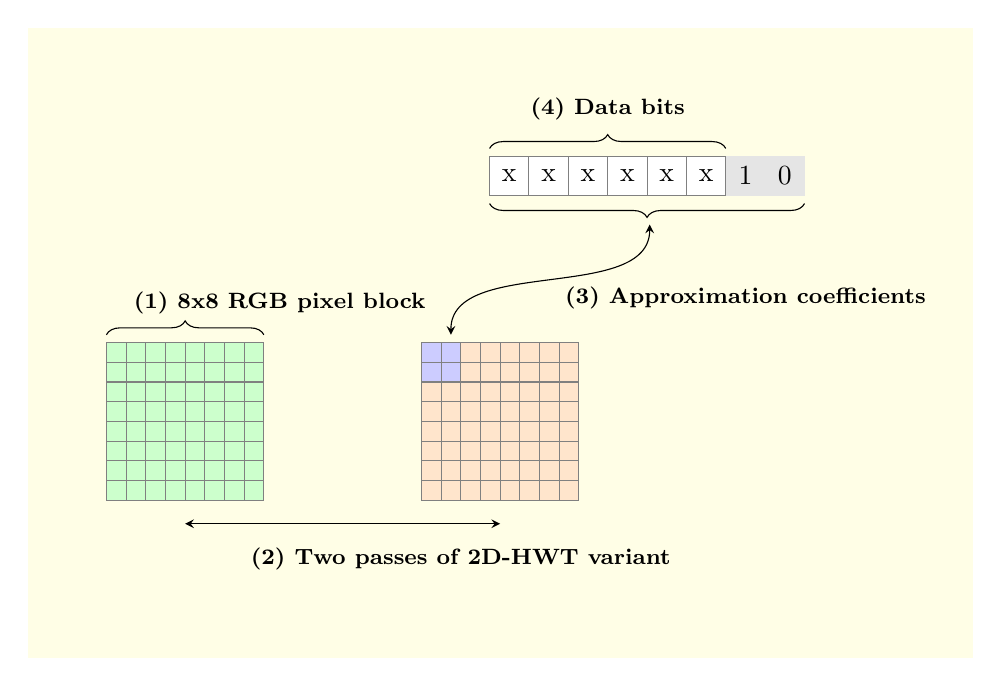
\begin{tikzpicture}[]


% bg bg

\fill[fill = yellow!10] (-2,-2) rectangle (10,6);

% bg
\fill[fill = green!20] (-1,0) rectangle (1,2);

\fill[fill = orange!20] (3-0.0001,0) rectangle (5,2);
\fill[fill = blue!20] (3-0.0001,1.5) rectangle (3.5,2);


% grids
\draw[step=0.25,color=black!50!white] (-1,0) grid (1,2);
\draw[step=0.25,color=black!50!white] (3-0.0001,0) grid (5,2);

% bits
\fill[xshift=110, yshift=110, fill = white] (3,0) (0,0) rectangle (4,0.5);
\draw[xshift=110, yshift=110, step=0.5,color=black!50!white, fill=white] (0,0) grid (4,0.5);



\draw[xshift=110, yshift=110] node at (0.25,0.25) {x};
\draw[xshift=110, yshift=110] node at (0.75,0.25) {x};
\draw[xshift=110, yshift=110] node at (1.25,0.25) {x};
\draw[xshift=110, yshift=110] node at (1.75,0.25) {x};
\draw[xshift=110, yshift=110] node at (2.25,0.25) {x};
\draw[xshift=110, yshift=110] node at (2.75,0.25) {x};

\draw [decorate,decoration={brace,amplitude=5pt}]
   (-1,2.1) -- (1,2.1);
\draw [decorate,decoration={brace,amplitude=5pt},xshift=110, yshift=110]
   (0,0.6) -- (3,0.6);
\draw [decorate,decoration={brace,amplitude=5pt},xshift=110, yshift=110]
   (4,-0.1) -- (0,-0.1);

\fill[xshift=110, yshift=110, fill = black!10!white] (3,0) rectangle (4,0.5);

\draw[xshift=110, yshift=110] node at (3.25,0.25) {1};
\draw[xshift=110, yshift=110] node at (3.75,0.25) {0};


% arrows

\draw[font={\footnotesize \bfseries}] node at (1.2,2.5) {(1) 8x8 RGB pixel block};


\draw[<->,>=stealth] (0,-0.3) -- (4,-0.3);
\draw[font={\footnotesize \bfseries}] node at (3.5,-0.75) {(2) Two passes of 2D-HWT variant};

\draw[<->,>=stealth] (3.375,2.1) .. controls (3.375,3.1) and (5.9,2.5) .. (5.9,3.5);
\draw[xshift=110, yshift=110, font={\footnotesize \bfseries}] node at (3.25,-1.3) {(3) Approximation coefficients};

\draw[xshift=110, yshift=110, font={\footnotesize \bfseries}] node at (1.5,1.1) {(4) Data bits};


\end{tikzpicture}
    
    \caption{Outline of the encoding process}
    \label{tikz:haar}
\end{center}
\end{figure}

The CImg class does contain Haar transforms but these are not suitable. We require an integer lifting scheme (described in \cite{haar}) to ensure that the transform is reversible. In the 1-dimensional case, for a pair of approximation and difference coefficients $(c_a,c_d)$, we calculate the output value pair $(x,y)$: 

\begin{eqnarray}
    x = & c_a + \lfloor \frac{c_d+1}{2} \rfloor \nonumber \\ 
    y = & x - c_d
\end{eqnarray}

Iteration of the above over pairs in both vertical and horizontal axis can be used to perform the full 2D HWT and its inversion losslessly.

Changing the approximation coefficients can also lead to capping of values as they are mapped back to greyscale space, outside the 0-255 range. We therefore selectively discard high frequency information (during the inverse transform) from the difference coefficient $c_d$ whenever capping occurs - leaving the approximation coefficients intact and the output within range. See appendix XXX for full details of the exact HWT variant used.



\FloatBarrier
\subsection{N-bit scaling}

The abstract base class {\tt ScaledConduitImage} contains functions to code n-bits of data to and from a single pixel using the n-bit scaling method. The value of n is set on instantiation.

Two subclasses are specified for $n=3$ and $n=4$. For $n=3$ we use 3x2 blocks of pixels with a block size of 3-bytes. For $n=4$ we use blocks of 2 pixels with a block size of 1-byte.

The scaling process works so that the intervals for each data point are of equal width, except for the intervals at either end which are $\frac{1}{2}$ length. This is because extreme values (0 or 255) can only be either decreased or increased due to compression artifacts, not both. An input pixel value of 255 might result in 254 or 253 after compression, but never 0 or 1.

    
\begin{figure}[htp]
  \begin{center}
    \subfigure[{\it HWT method}]
        {\label{fig:edge-a}\includegraphics[width=4cm]{screens/haar.jpg}}
    \subfigure[{\it 3-bit scaling method}]
        {\label{fig:edge-b}\includegraphics[width=4cm]{screens/scaled3.jpg}}
    \subfigure[{\it 4-bit scaling method}]
        {\label{fig:edge-b}\includegraphics[width=4cm]{screens/scaled4.jpg}}
  \end{center}
  \caption{Final output of the image coding process.}
  \label{scn:images}
\end{figure}
    

\FloatBarrier
\section{Testing}

Many modules or processes could be unit tested individally before being aggregated and integration testing performed. Note that this section does not describe the chronology of development. In accordance with an agile developmental approach the focus was on delivering a minimally functioning prototype as earlier in the development lifecycle as possible, combining aspects of all the components listed below. Iterative improvement and development was then performed until a fully functioning system emerged.


\subsection{Page interception module}

The {\tt pagecept} parsing module was present in early prototypes, with placeholder messages and images used to demarcate decrypted items and skeleton handlers attached to UI controls. Testing principally involved manual inspection of the DOM using FireBug to ensure parsing had occured correctly. Test scripts derived from boundary-value analysis (available in appendix XXX) were also ran using FireBug and FireUnit to test that DOM insertions were being sanitised correctly. The cognitive walkthough method was also performed periodically to identify useability issues with UI controls, which could then be fixed.

Initially a small subset of decryption target types and control-input pairs were supported. As development progressed each sucessive prototype added wider support for more specific cases. Testing was tightly integrated with and performed thoughout development, in line with agile testing methedology.


\subsection{Image coding}

Development of image coding algorithms, particularly the HWT method, was highly suseptible to conceptual bugs, whereby the only error indicator was higher than expected output error rates. Error rates had to be carefully monitored during development. Testing involved simulating compression using the IGJ {\tt libjpeg} library --- initially for single $8 \times 8$ blocks then later for entire images. Debug methods were created for calculating the Hamming distance, edit distance and other metrics between byte sequences and/or files.


\subsection{Other modules}

The UTF-8 codec was also tested using boundary-value analysis (available in appendix XXX). A standalone test instance of the C++ library was used since starting and stopping the browser was considerably time consuming.

Layers of encoding for both text and images were added to successive prototypes. Encoding layers could then be turned on and off during testing with command line switches to isolate bugs to specific library components.


\subsection{Integration testing}

Eventually simulation of the JPEG compression process was replaced by automated uploading and dowloading of images to and from Facebook.

Particular care was taken to ensure text sanitisation was tested end-to-end, including submission and retriveal to/from Facebook, since the complexity of the UTF-8 coding scheme and the custom built decoder introduced the possibility of bypassing sanitisation \cite{utf8}.\footnote{Since we sanitise before injecting anything in to the page, in retrospect it seem unlikely that this could ever be a problem.}
